% Strona tytułowa referatu ze względu na możliwe odmienne parametry formatowania
% znajduje się w oddzielnym pliku prezentacja_tytul.tex
% Tutaj powtórzony tytuł i autorzy, by było w informacjach o pliku
% Tytuł referatu
\title{Tytuł prezentacji}
% Autor referatu
\author{Autorzy} 
% Data
%\date{}
%\date[23 września 2009 roku]{Wrocław, 23 września 2009 roku}
\date[\today]{Wrocław, \today}

% Ustawienia pakietu hyperref - lista możliwych pozycji na
% http://en.wikibooks.org/wiki/LaTeX/Hyperlinks i w dokumentacji hyperref
\hypersetup{unicode=true,
  pdftitle={Przykład prezentacji w beamerze zgodnej
    z logotypem PWr i KCiR (W4/K7)},
  pdfauthor={Robert Muszyński},
  pdfsubject={Prezentacja w~ramach Konferencji...},
  linkcolor=tango, urlcolor=tango}

% Ścieżka do katalogu z obrazkami
\graphicspath{{./Obrazki/}}
\usepackage{multicol}
\begin{document}

% \setbeamercovered{transparent}

% Strona tytułowa
% pdf wyprodukowany na podstawie oddzielnego pliku opisującego
% stronę tytułową przy innym formatowaniu

 {
   \setbeamercolor{background canvas}{bg=}
   \setbeamertemplate{navigation symbols}{} %remove navigation symbols
   
\includepdf[pages=1]{prezentacja_tytul.pdf}
 }

% % alternatywny sposób dołączenia strony tytułowej tak, by była w ramce
% % (potrzebne, gdy mamy notatki poza frame'ami i używamy 
% % opcji ignorenonframetext) ale coś nie tak z poziomym ułożeniem
% % (stąd poniżej dodatkowy hspace po 3 standardowych)
% {
%   \hspace*{-\hoffset}
%   \hspace*{-1in}
%   \hspace*{-\oddsidemargin}
%   \hspace*{-6.45mm}
%   \setbeamertemplate{navigation symbols}{}%remove navigation symbols
%   \frame[plain]{
\includegraphics[page=1,width=\paperwidth]{prezentacja_tytul.pdf}}
% }

%% Spis treści
 \section*{Plan prezentacji}
 \begin{frame}%[plain]
   \frametitle{Plan prezentacji}
   \tableofcontents[hidesubsections]%,pausesections]
 \end{frame}
\section{Wprowadzenie}

\section{Założenia projektowe}
\begin{frame}
\frametitle{Co robot powinien posiadać?}
\begin{block}{Robot powinien:}
\begin{enumerate}
\setlength{\itemsep}{2mm}
\item Posiadać wirujące szczotki myjące podłogi
\item Posiadać system dozujący wodę z detergentem
\item Posiadać system zbierający zużytą wodę z podłogi
\item Potrafić rozpoznawać przeszkody
\item Potrafić rozpoznawać niebezpieczne różnice wysokości podłogi
\item Posiadać system jezdny pozwalający łatwo osiągać zadane położenia
\item Posiadać możliwość określania swojej bieżącej pozycji
\item Sygnalizować zdarzenia nadzwyczajne
\end{enumerate}
\end{block}
\end{frame}

\begin{frame}
\frametitle{Wybór klasy robota}
\begin{block}{Robot klasy 2,0}
\begin{enumerate}
\setlength{\itemsep}{2mm}
\item prostota sterowania
\item prostota konstrukcji
\item obrót w miejscu
\item wrażliwość na nierówności
\end{enumerate}
\end{block}
\begin{block}{Sterowanie}
	\begin{enumerate}
		\item Sterowanie TYLKO kinematyczne
		\item Kontroler kinematyczny - algorytm Samsona
	\end{enumerate}
\end{block}
\end{frame}

\section{Konstrukcja}

\begin{frame}
\frametitle{Podzespoły}
\scriptsize
\begin{minipage}{0.45\textwidth}
\begin{block}{Mikrokontroler: STM32F103C8T6 - Blue Pill}
\begin{center}
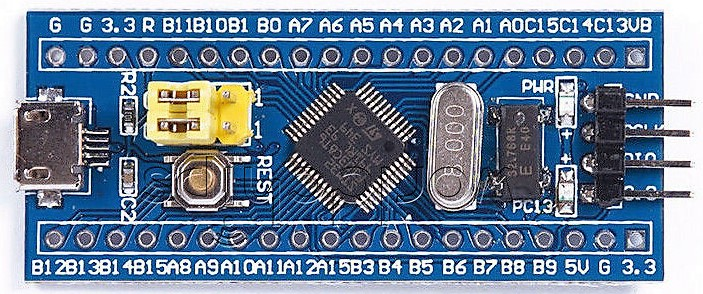
\includegraphics[scale=0.22]{bluepill.jpg}\hspace{12mm}
\end{center}
\end{block}
\end{minipage}
\hspace{5mm}
\begin{minipage}{0.45\textwidth}
\begin{block}{Pomiar odległości od podłogi}
	Czujnik IR i komparatorem LM393
	\begin{center}
		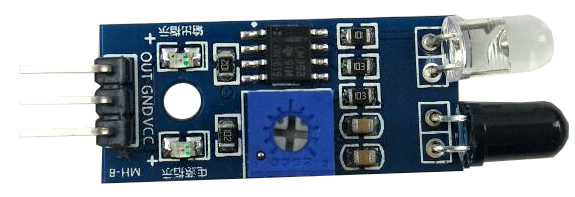
\includegraphics[scale=0.22]{czujnikIR.png}\hspace{12mm}
	\end{center}
\end{block}
\end{minipage}
\begin{block}{Detekcja kolizji}
	Bumper wykonany z 2 wyłączników krańcowych.
\end{block}
\begin{block}{Komunikacja z użytkownikiem}
	\begin{minipage}{0.49\textwidth}
	Przyciski:
	\begin{itemize}
		\item Start/Stop
		\item Włącz/Wyłącz
	\end{itemize}
\end{minipage}
\begin{minipage}{0.49\textwidth}
	Sygnalizacja zdarzeń:
	\begin{itemize}
		\item Buzzer
	\end{itemize}
\end{minipage}
\end{block}
\end{frame}

\begin{frame}
\frametitle{Podzespoły - cd}
\begin{block}{Silniki DC z przekładnią}
	\begin{minipage}{0.39\textwidth}
\begin{center}
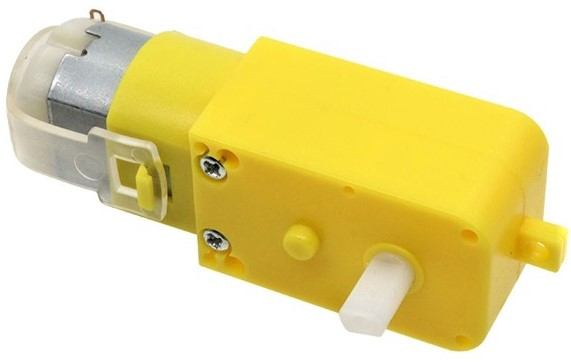
\includegraphics[scale=0.22]{silnikDC.jpg}\hspace{12mm}
\end{center}
\end{minipage}
\begin{minipage}{0.59\textwidth}
Prędkość -- 100 obr/min. W testach praktycznych nawet 200 obr/min
\end{minipage}
\end{block}



\begin{block}{Enkodery}
	\begin{minipage}{0.39\textwidth}
\begin{center}
	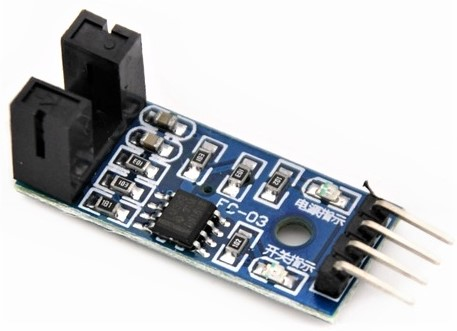
\includegraphics[scale=0.2]{enkoder.jpg}\hspace{12mm}
	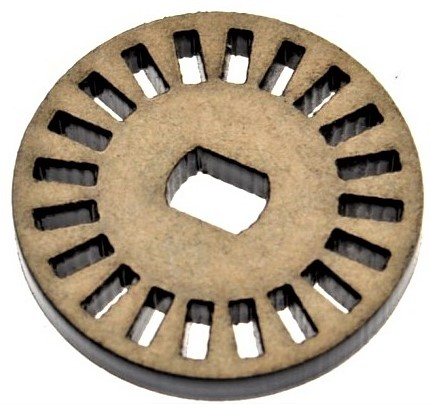
\includegraphics[scale=0.1]{plytkaEnkodera.jpg}   
\end{center}
\end{minipage}
\begin{minipage}{0.59\textwidth}
	Enkoder optyczny mocowany do wału silnika. Płytka szczelinowa posiada rozdzielczość 20 linii na obrót. Badając oba zbocza mam 40 impulsów na obrót, a z uwzględnieniem przekładni wbudowanej w silnik $48 * 40 = 1920$. 
\end{minipage}
\end{block}



\end{frame}

\begin{frame}
\frametitle{Podzespoły - cd}
\begin{block}{Zasilanie}
\begin{itemize}
\item 2 akumulatory Li-Ion 18650 połączone szeregowo. Napięcie nominalne pakietu 7.4~V
\item 2 przetwornice Step-Down. Prąd ciągły maksymalny 1.8~A
\item Zabezpieczenie moduł BMS
\end{itemize}
\end{block}
\begin{block}{Układy pompujące wodę}
	\begin{minipage}{0.49\textwidth}
		Zraszanie podłogi -- pompka odśrodkowa
		\begin{center}
			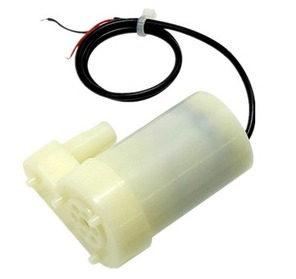
\includegraphics[scale=0.2]{pompka.jpg}\hspace{12mm} 
		\end{center}
	\end{minipage}
	\begin{minipage}{0.49\textwidth}
		Zasysanie brudnej wody - pompka membranowa
		\begin{center}
			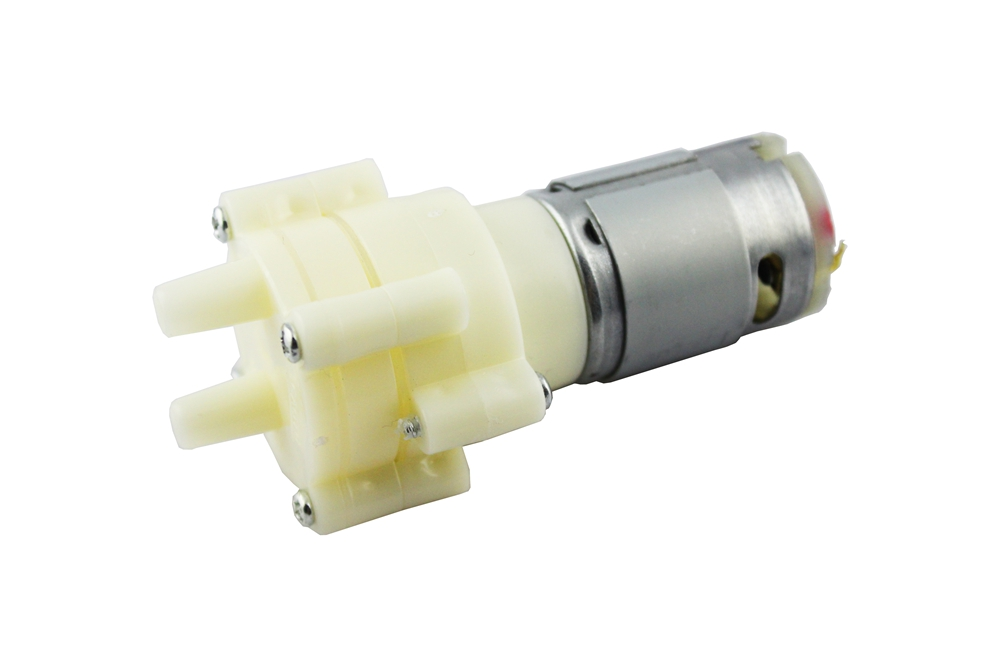
\includegraphics[scale=0.35]{rys/membranowa.jpg}\hspace{12mm} 
		\end{center}
	\end{minipage}
\end{block}
\end{frame}

\section{Teoria}

\section{Software}
\begin{frame}
\frametitle{Wykorzystany software i styl pisania kodu}
\tiny
Software:
\begin{enumerate}
\item IDE: PlatformIO w połączeniu z CLion oraz VS Code
\item Symulacje: Matlab oraz Simulink
\item Schematy: Altium Designer
\item Rysunki: Inkscape
\item Graficzna prezentacja danych: 
\begin{itemize}
	\tiny
	\item Processing (wizualizacja w czasie rzeczywistym)
	\item Python + Matplotlib (cały przebieg)
\end{itemize}
\end{enumerate}
Styl pisania kodu:
		\begin{itemize}
			\item Kod pisany obiektowo. Ostatecznie 18 klas.
			\item Dzięki obiektowemu podejściu możliwość przeciążenia operatora \texttt{<<} (łatwy debug).
			\item Standard C++11 -- przydomek \texttt{constexpr}.
			\item \texttt{-Wall}, \texttt{-Wextra}.
			\item Makro \texttt{F()} -- ciągi w flash zamiast RAM.
		\end{itemize}
		Problemy:
		\begin{itemize}
			\item Framework nie jest najlepiej napisany. Użycie \texttt{-Wall -Wextra -O3} powoduje dużo warningów.
			\item Błędy kompilacji -- użycie zmiennej statycznej w złym miejscu powoduje \SI{3}{x} wzrost objętości programu i przekroczenie dostępnej pamięci. W jednym przypadku konieczne było użycie git reset.
			\item CLion nie jest przystosowany do PlatformIO - czasami się psuje.
		\end{itemize}
		Sumarycznie jednak zaoszczędzony czas w zupełności wynagrodził te problemy.
\end{frame}
\section{Kinematyka robota}

\begin{frame}
  	\frametitle{Obliczenia}  
  	\tiny
	\begin{block}{Ograniczenia w postaci Pfaffa}
		\begin{equation*}
			A(q)\dot{q} =
			\begin{bmatrix*}[r]
				sin(\varphi) & -cos(\varphi) & 0  &  0 & 0 \\
				cos(\varphi) & sin(\varphi)  & -l & -R & 0 \\
				cos(\varphi) & sin(\varphi)  & l  &  0 & -R 
			\end{bmatrix*}
			\left(\begin{array}{c}
				\dot{x} \\ \dot{y} \\ \dot{\varphi} \\ \dot{\phi}_1 \\ \dot{\phi}_2
			\end{array}\right)
		\end{equation*}
	\end{block}
	\begin{block}{Bezdryfowy układ sterowania}
		\begin{minipage}{0.49\textwidth}
			\begin{equation*}
			\dot{q} = G(q)\eta =
			\begin{bmatrix*}
			cos(\varphi) & cos(\varphi) \\
			sin(\varphi) & sin(\varphi) \\
			\frac{1}{l} & -\frac{1}{l} \\
			\frac{2}{R} & 0 \\
			0 & \frac{2}{R} 
			\end{bmatrix*}
			\left(\begin{array}{c}
			\eta_1 \\
			\eta_2
			\end{array}\right),
			\end{equation*}
		\end{minipage}
	%\hspace{1cm}
		\begin{minipage}{0.49\textwidth}
			\begin{equation*}
			\left(\begin{array}{c}
			\dot{x} \\
			\dot{y} \\
			\dot{\varphi}
			\end{array}\right)
			=
			\begin{bmatrix}
			cos(\varphi) & 0 \\
			sin(\varphi) & 0 \\
			0 & 1
			\end{bmatrix}
			\left(\begin{array}{c}
			v \\
			\omega
			\end{array}\right)
			\end{equation*}
		\end{minipage}
	\end{block}
	\begin{block}{Algorytm Samsona}
		\begin{equation*}
		\left(\begin{array}{c}
		v_{r} \\
		\omega_{r} 
		\end{array}\right)
		=
		\left(\begin{array}{c}
		k_{1}x_{e} + v_{d}cos(\varphi_{e}) \\
		\omega_{d} + k_{2}\varphi_{e} + v_{d}y_{e}\frac{sin(\varphi_{e})}{\varphi_{e}}
		\end{array}\right)
		\end{equation*}
	\end{block}
\end{frame}

\section{Symulacje sterownika kinematycznego}
	\begin{frame}
	\frametitle{Test generowania trajektorii jazdy po pokoju}  
		Wykonany dla parametrów $k1$ i~$k2$ odpowiednio $0.1$ oraz $1$:
		\begin{center}
			\includegraphics[width=0.49\textwidth]{rys/trajektoriaRownoleglek1=02k2=10s1.eps}
			\includegraphics[width=0.49\textwidth]{rys/trajektoriaKwadratk1=02k2=10s1.eps}  
		\end{center}
	\end{frame}

	\begin{frame}
	\frametitle{Porównanie wpływu parametru k1 i k2}  
		\begin{center}
			\includegraphics[width=0.38\textwidth]{rys/trajektoriaRownoleglaPorownaniek1.eps}
			\includegraphics[width=0.38\textwidth]{rys/trajektoriaKwadratPorownaniek1.eps}  
		\end{center}
	\begin{center}
		\includegraphics[width=0.38\textwidth]{rys/trajektoriaRownoleglaPorownaniek2.eps}
		\includegraphics[width=0.38\textwidth]{rys/trajektoriaKwadratPorownaniek2.eps}  
	\end{center}
	\end{frame}

	\begin{frame}
	\frametitle{Czy ta realizacja jest możliwa?}  
	\tiny
		Aby wiedzieć czy robot jest w stanie to zrealizować należy sprawdzić prędkości obrotowe kół. Dla kolejnych symulacji $k1 = 1, k2 = 2$. Prędkość obrotowa silników to \SI{100}{obr\per\second} czyli $1\frac{2}{3}$\si{obr\per\second}.
		\begin{center}
			\includegraphics[width=0.35\textwidth]{rys/trajektoriaRownoleglek1=1k2=10.eps}
			\includegraphics[width=0.35\textwidth]{rys/predkosciKolRownoleglek1=1k2=10.eps}  
		\end{center}
	\begin{center}
		\includegraphics[width=0.35\textwidth]{rys/trajektoriaKwadratk1=1k2=10.eps}
		\includegraphics[width=0.35\textwidth]{rys/predkosciKolKwadratk1=1k2=10.eps}
	\end{center}
	\end{frame}

	\begin{frame}
	\frametitle{Jak to rozwiązać?}  
		Z poprzednich symulacji wynikało że największy problem generowały gwałtowne zmiany kierunku. Spróbujmy je wygładzić.
		\begin{center}
			\includegraphics[width=0.49\textwidth]{rys/trajektoriaRownoleglek1=1k2=10s=01d02LimitZaokraglone.eps}
			\includegraphics[width=0.49\textwidth]{rys/predkoscKolRownoleglek1=1k2=10s=01d02LimitZaokraglone.eps}
		\end{center}
		Jest dobrze. Prędkości kół nie osiągają wartości granicznych.
	\end{frame}

	\begin{frame}
	\frametitle{Problem z trajektorią do środka}  
		Aby sprawdzić co jest nie tak porównajmy kąt obrotu zadany z rzeczywistym.
		\begin{center}
			\includegraphics[width=0.49\textwidth]{rys/trajektoriaKwadratk1=1k2=10d02s01LimitZaokraglone.eps}
			\includegraphics[width=0.49\textwidth]{rys/katyKwadratk1=1k2=10d02s01LimitZaokraglone.eps} 
		\end{center}
		Widać, że robot zamiast gładko przejść do pozycji $2\pi$ odkręca się do pozycji $0$.
	\end{frame}

	\begin{frame}
	\frametitle{Rozwiązanie}  
		Choć pozycje $0$ i $2\pi$ są tym samym punktem w układzie współrzędnych, potrzebujemy dodatkowo informacji o ilościach obrotów. Najprościej to osiągnąć zmieniając zakres kąta obrotu z $\langle 0, 2\pi)$ do $(-\infty, +\infty)$.
		\begin{center}
			\includegraphics[width=0.45\textwidth]{rys/trajektoriaKwadratk1=1k2=10d02s01LimitZaokragloneNaprawione.eps} 
		\end{center}
	\end{frame}

\section{Rzeczywista implementacja}

	\begin{frame}
	\frametitle{Symulacja sterownika kinematycznego}  
		Parametry symulacji ustawiono na $k1 = 1$, $k2 = 1$. Prędkość robota \SI[per-mode=symbol]{10}{\centi\meter\per\second}. Prędkość transmisji \SI{7.2}{\mega Bd}. Kolor biały reprezentuje trajektorię zadaną, natomiast czerwony rzeczywistą. Dodatkowo dane logowane logowane do pliku \texttt{.txt}. Wyświetlane w skrypcie \texttt{Python} z użyciem biblioteki \texttt{Matplotlib}.
		\begin{center}
			\includegraphics[width=0.4\textwidth]{rys/trajektoriaProcessingk1=1k2=1.png}
			\includegraphics[width=0.49\textwidth]{rys/predkosciKolPythonk1=1k2=2.eps}
		\end{center}
		
	\end{frame}

	\begin{frame}
	\frametitle{Testy na rzeczywistym robocie}
	\begin{minipage}{0.24\textwidth}
	
		\begin{figure}
			\centering
			\includegraphics[width=\textwidth]{rys/otwartaPetla.png}
		\end{figure}
\end{minipage}
	\hspace{3mm}
	\begin{minipage}{0.65\textwidth}
		\begin{figure}
			\centering
			\includegraphics[width=\textwidth]{rys/zamknietaPetla.png}
		\end{figure}
	\end{minipage}
	\end{frame}

	\begin{frame}
	\frametitle{Ostateczne wyniki}
		\begin{figure}
			\centering
			\includegraphics[width=0.49\textwidth]{rys/trajektoriaPythonOstatnie.eps}
			\includegraphics[width=0.49\textwidth]{rys/predkosciKolPythonOstatnie.eps}
		\end{figure}
	Jeden z silników jest niskiej jakości i stawia nierówny opór. Jednak nie wpływa to znacząco na trajektorię.
	\end{frame}

\section{Testy elektroniki}

\begin{frame}
\frametitle{Drgania styków i filtracja zasilania} 
\begin{center}
	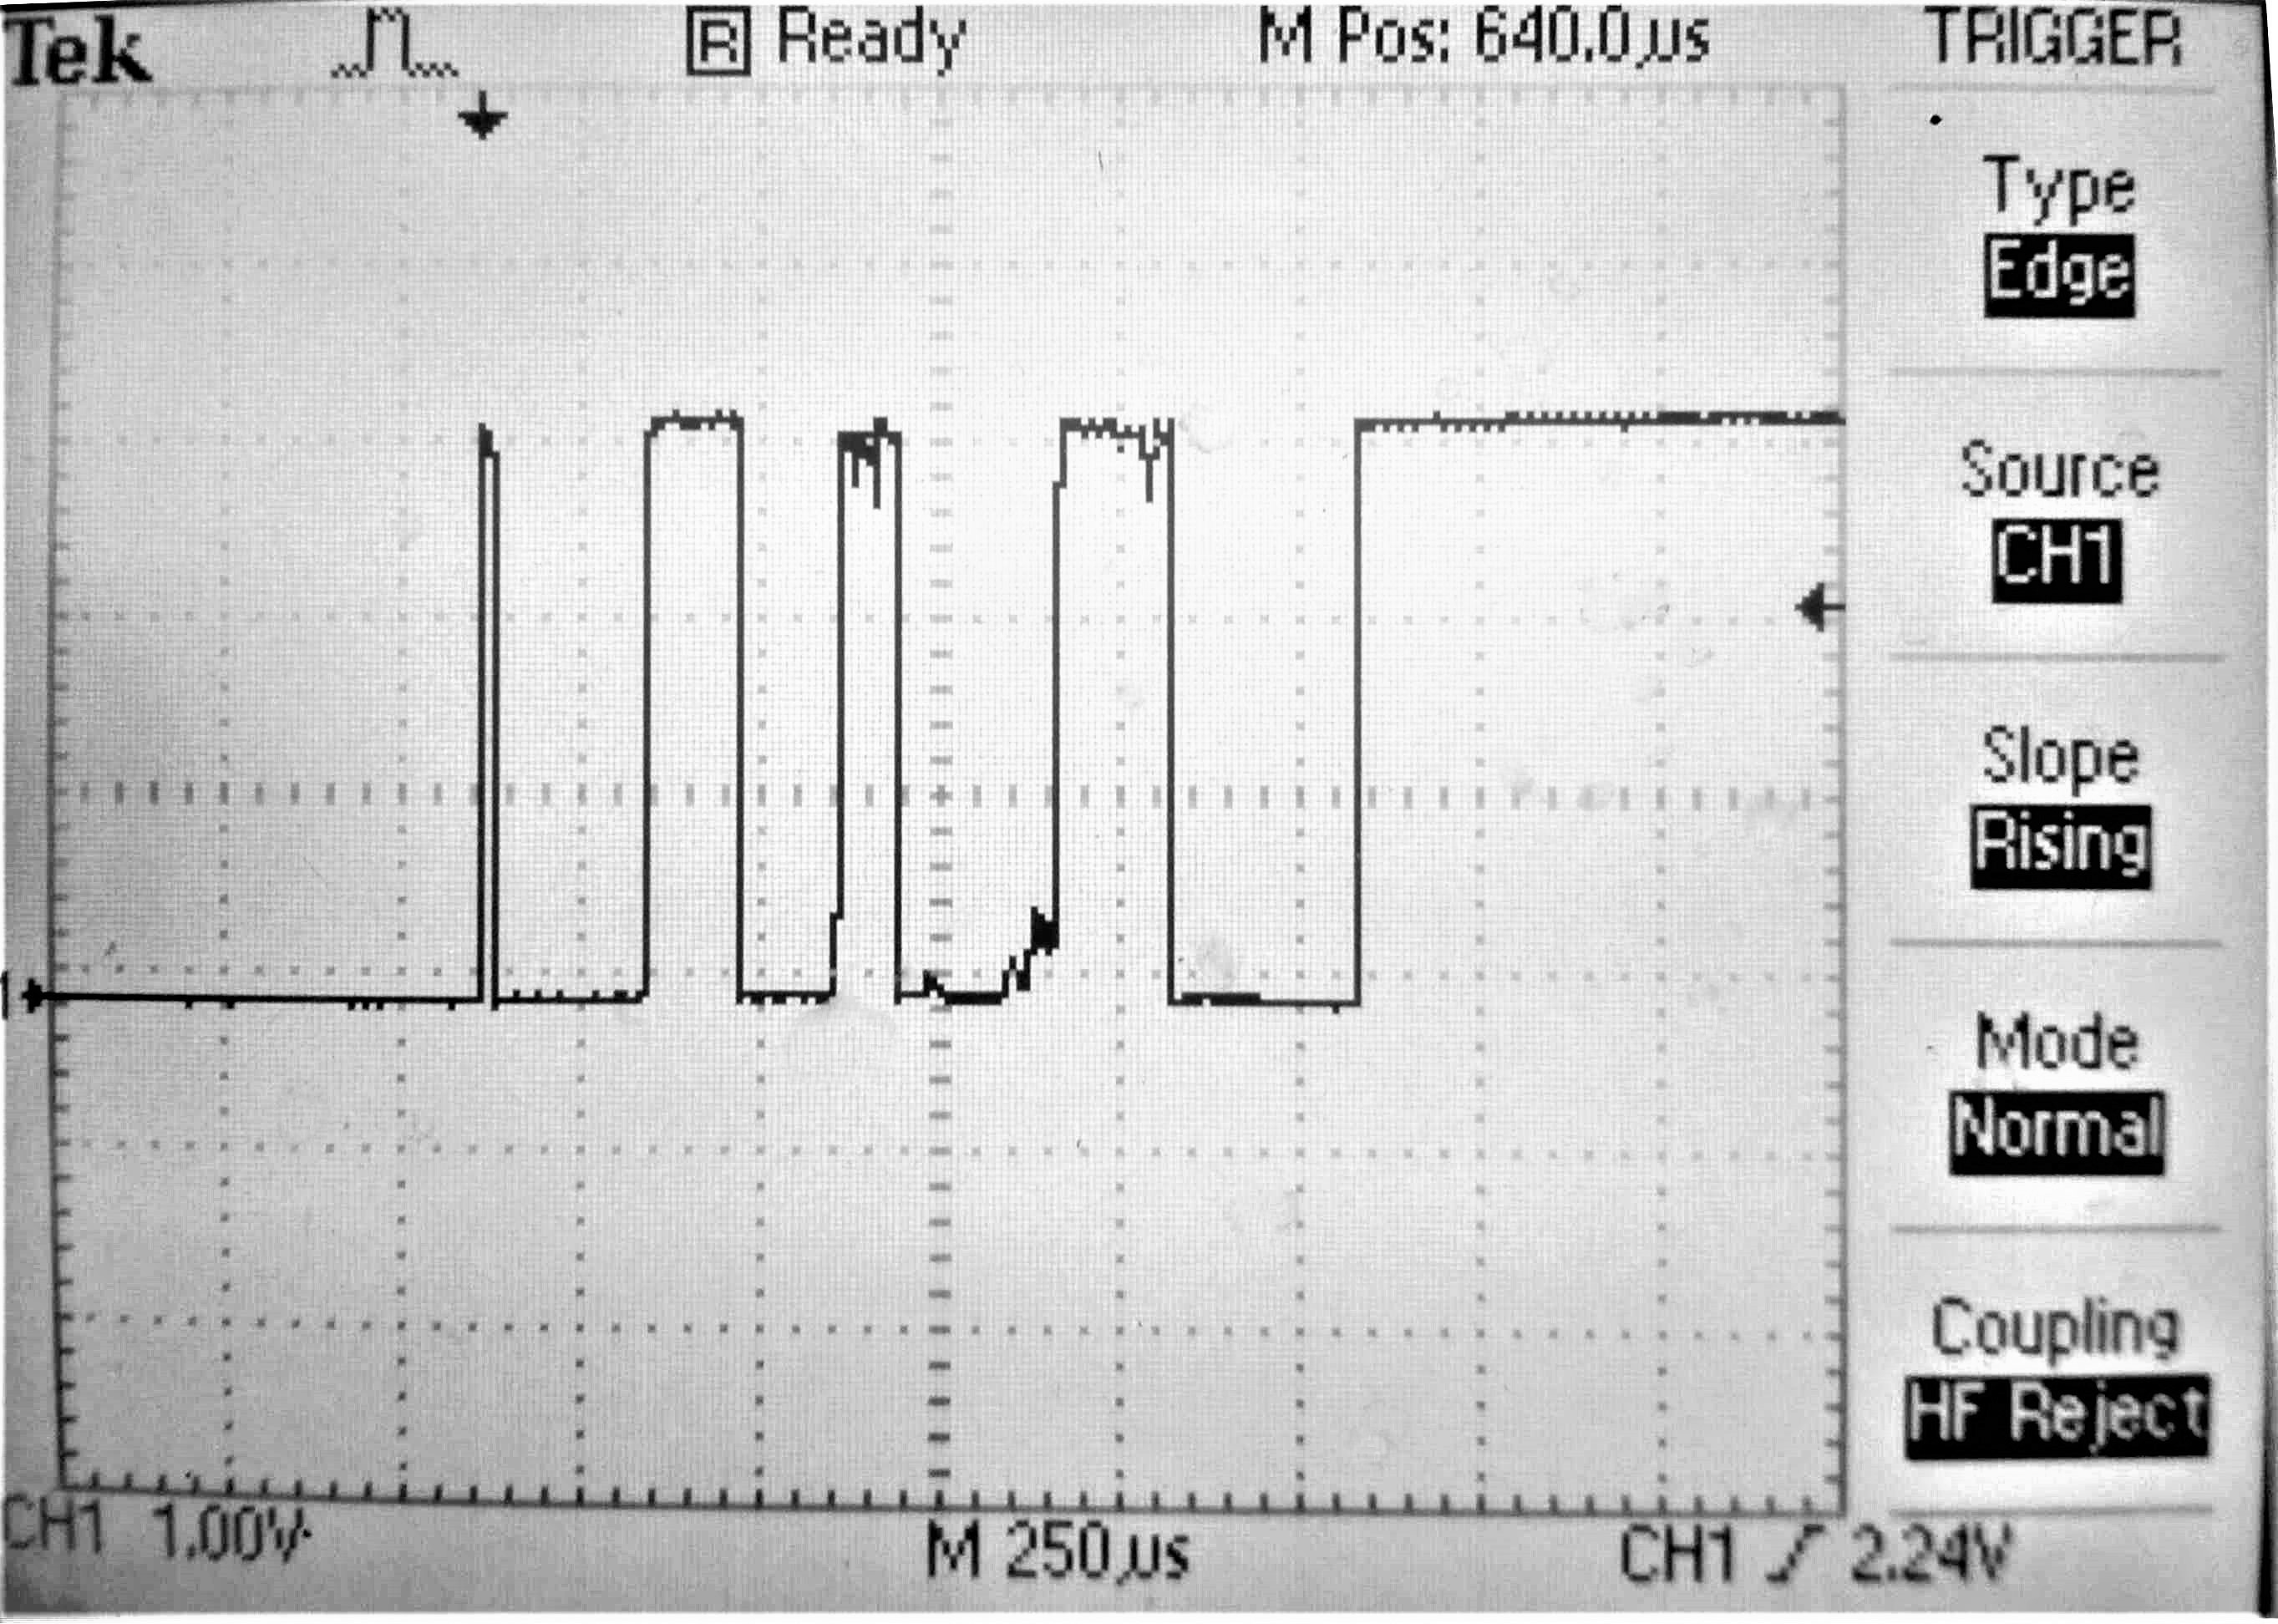
\includegraphics[width=0.39\textwidth]{rys/drganiaPrzyciskow.jpg}
	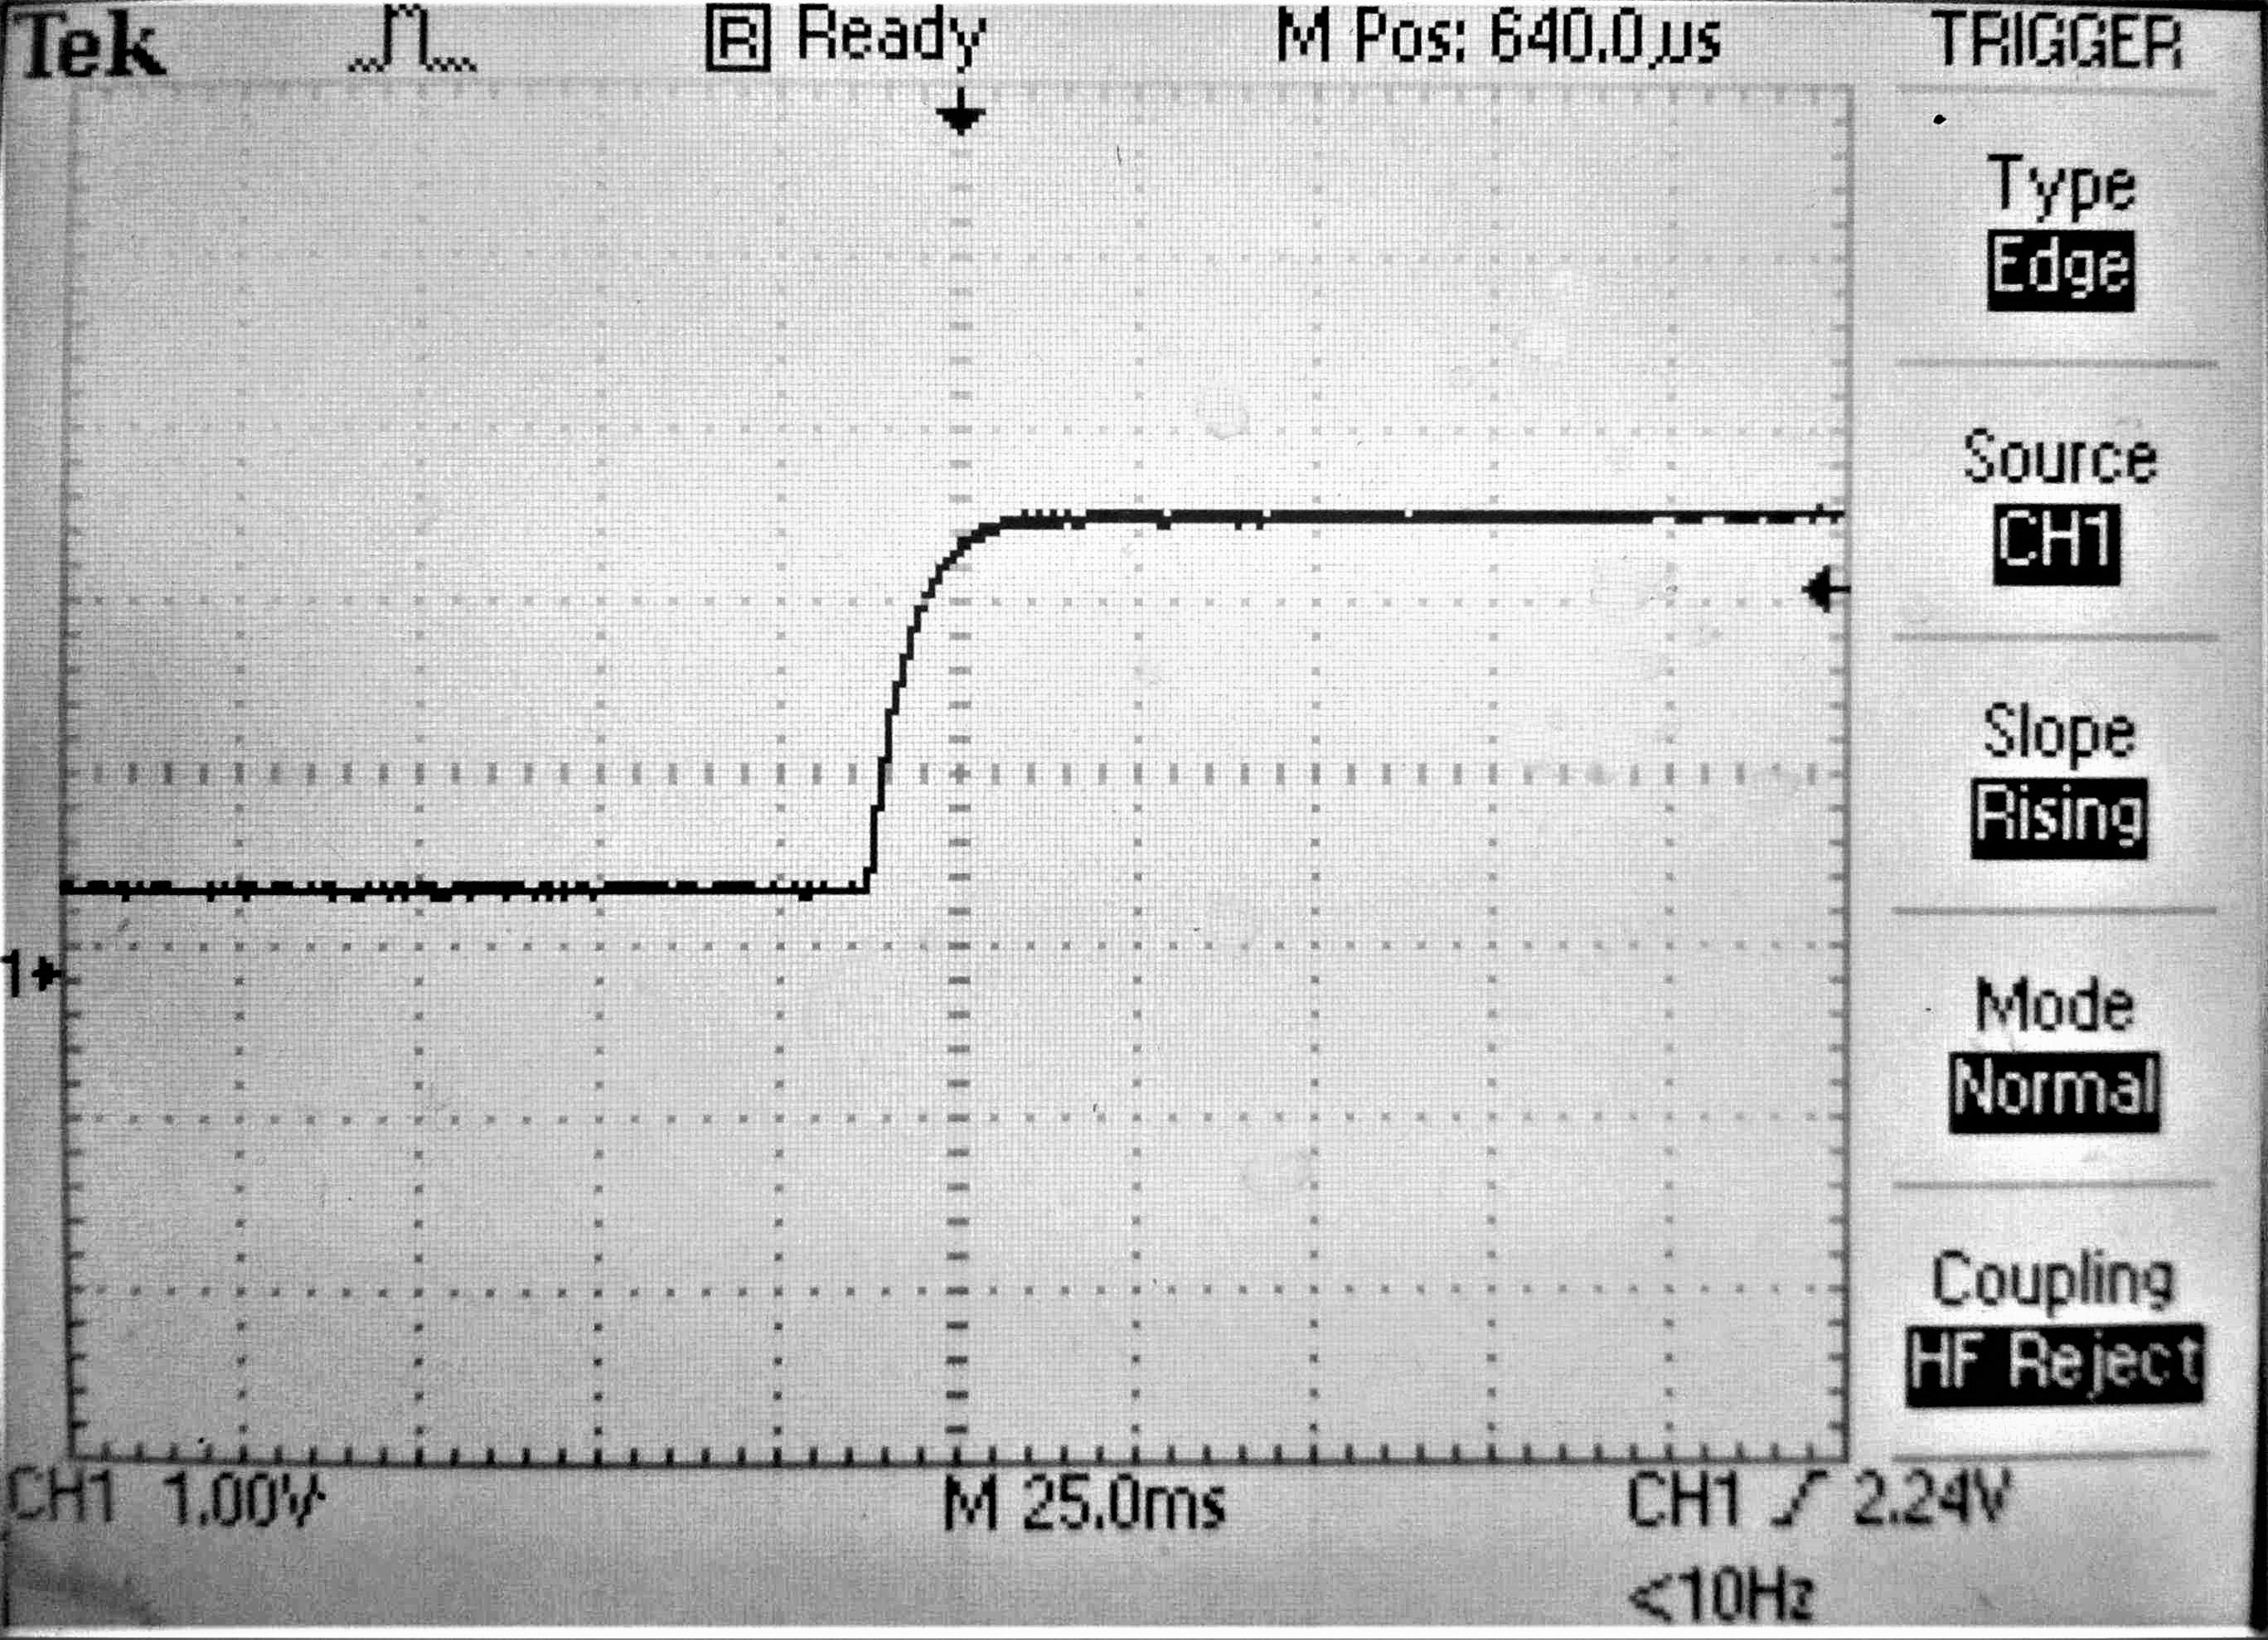
\includegraphics[width=0.39\textwidth]{rys/drganiaStykowFiltr.jpg}
\end{center} 
\begin{center}
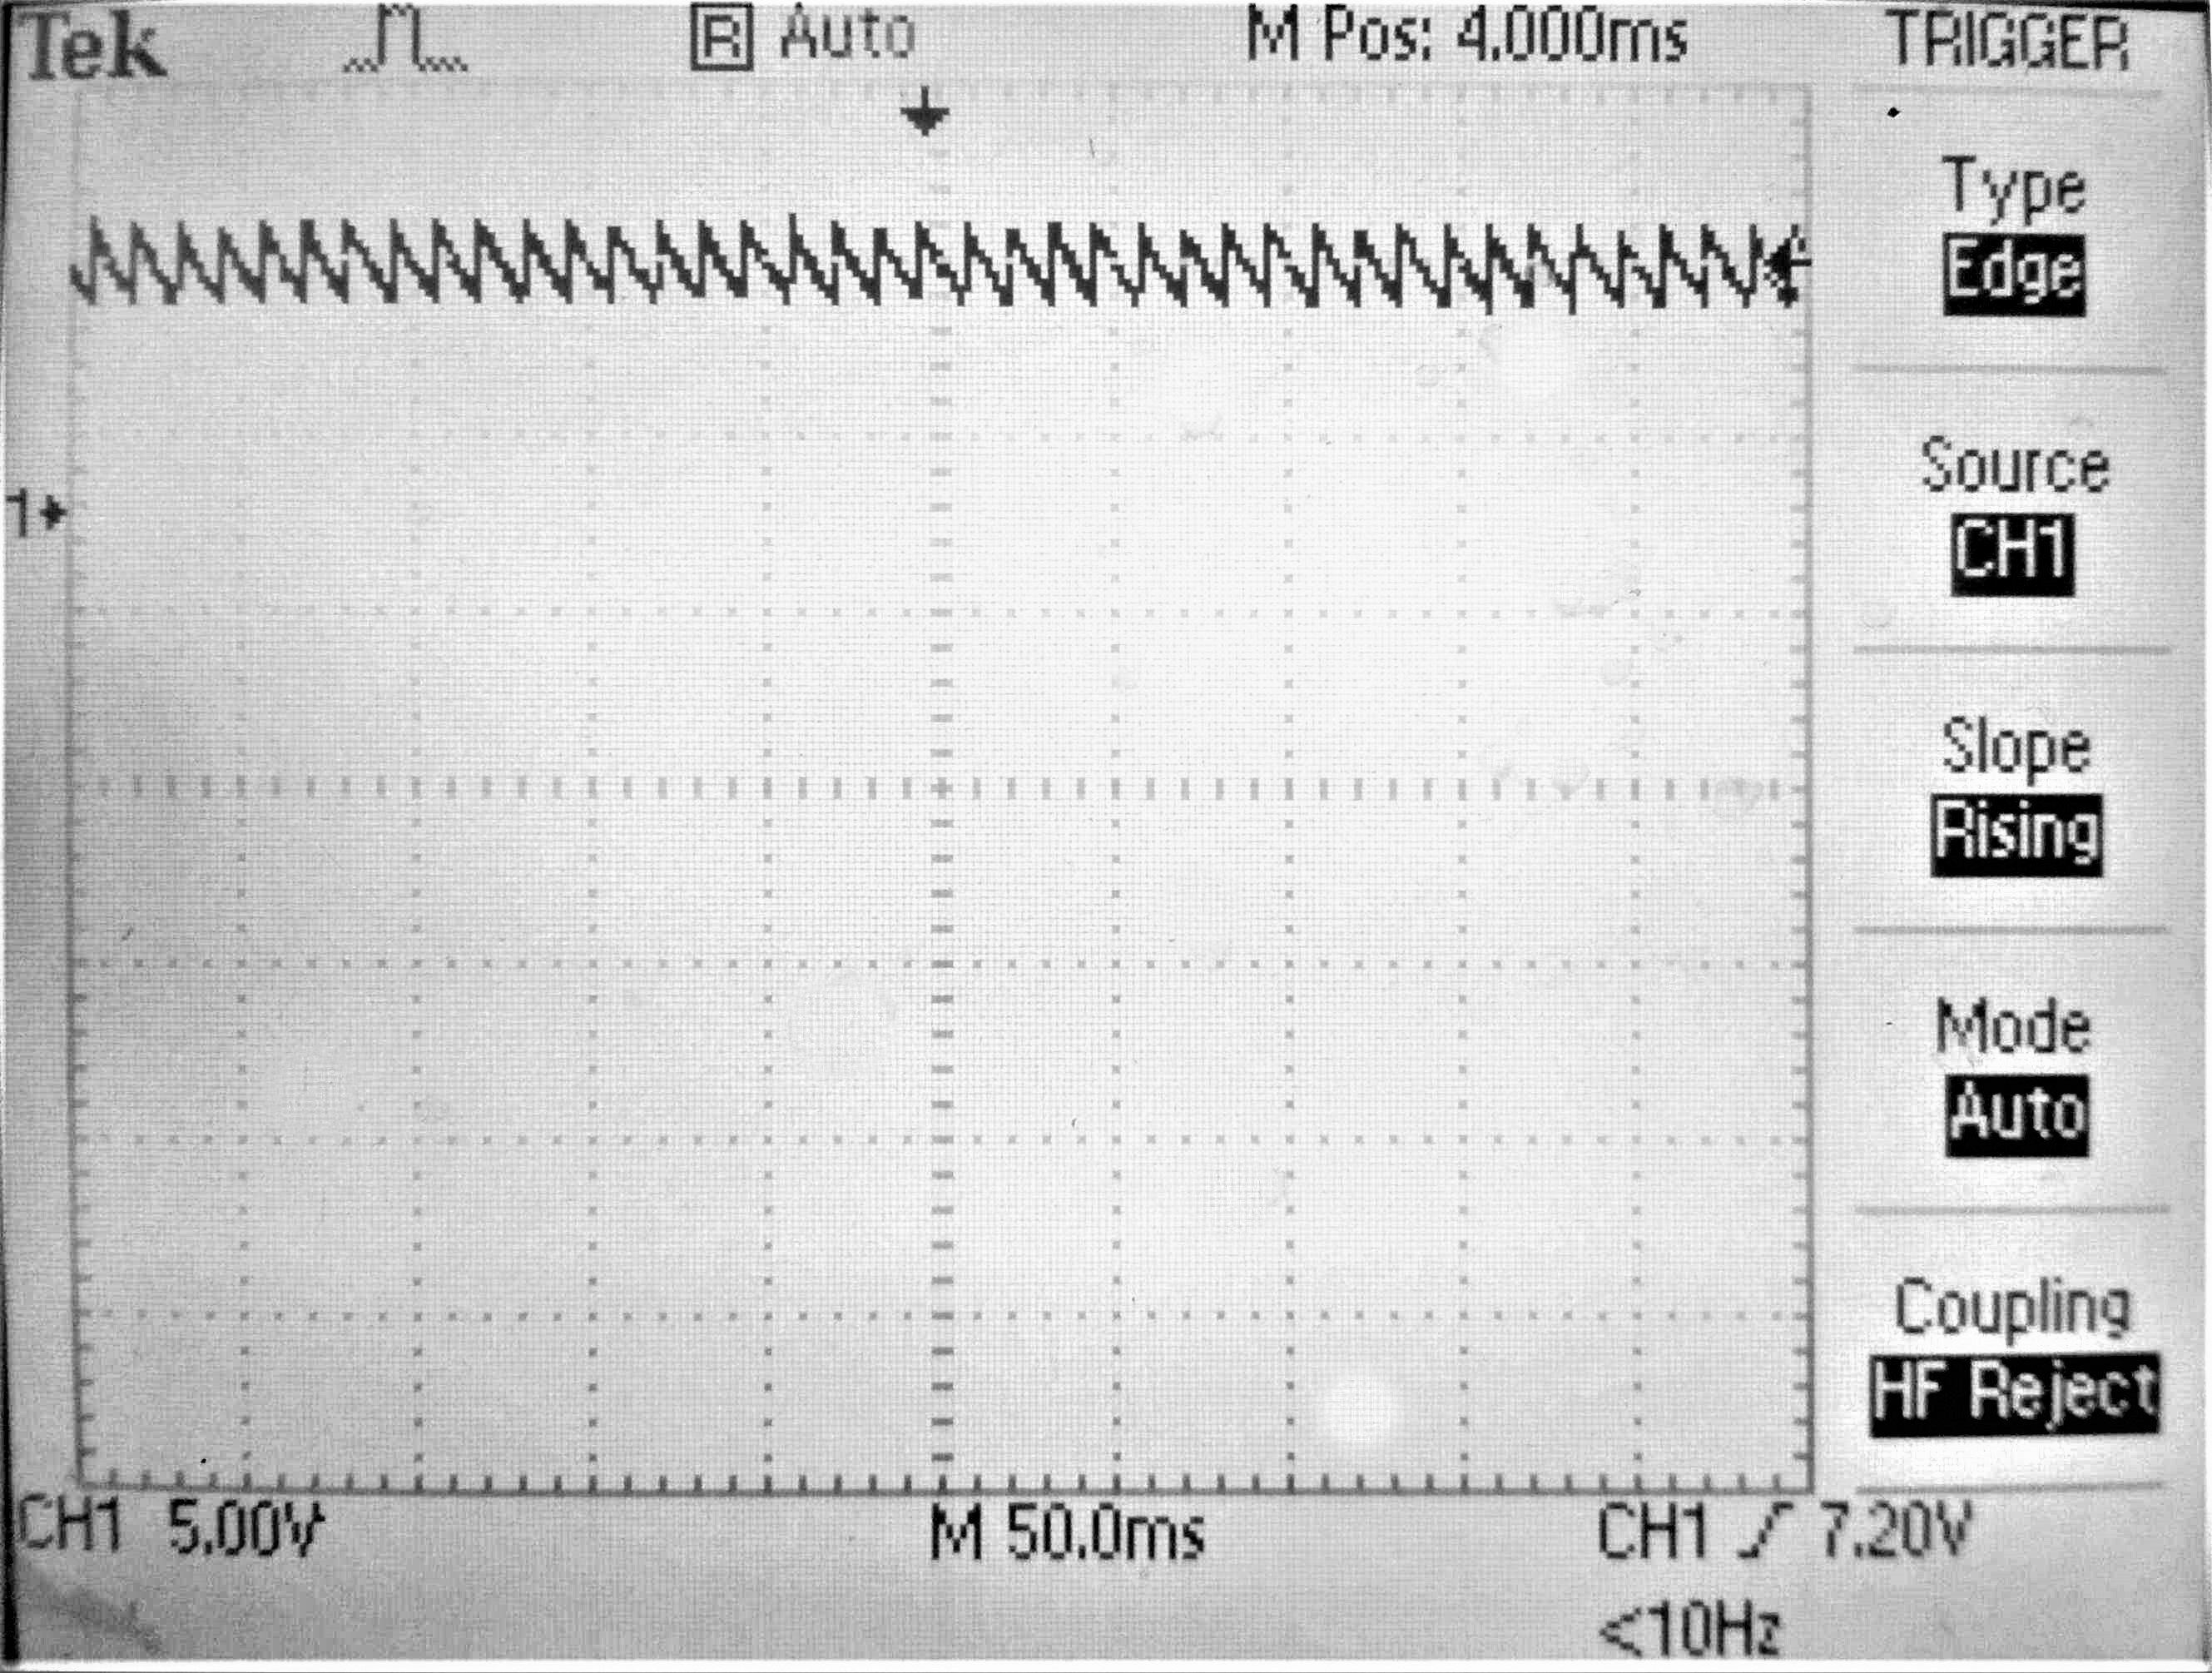
\includegraphics[width=0.39\textwidth]{rys/zasilanie.jpg} 
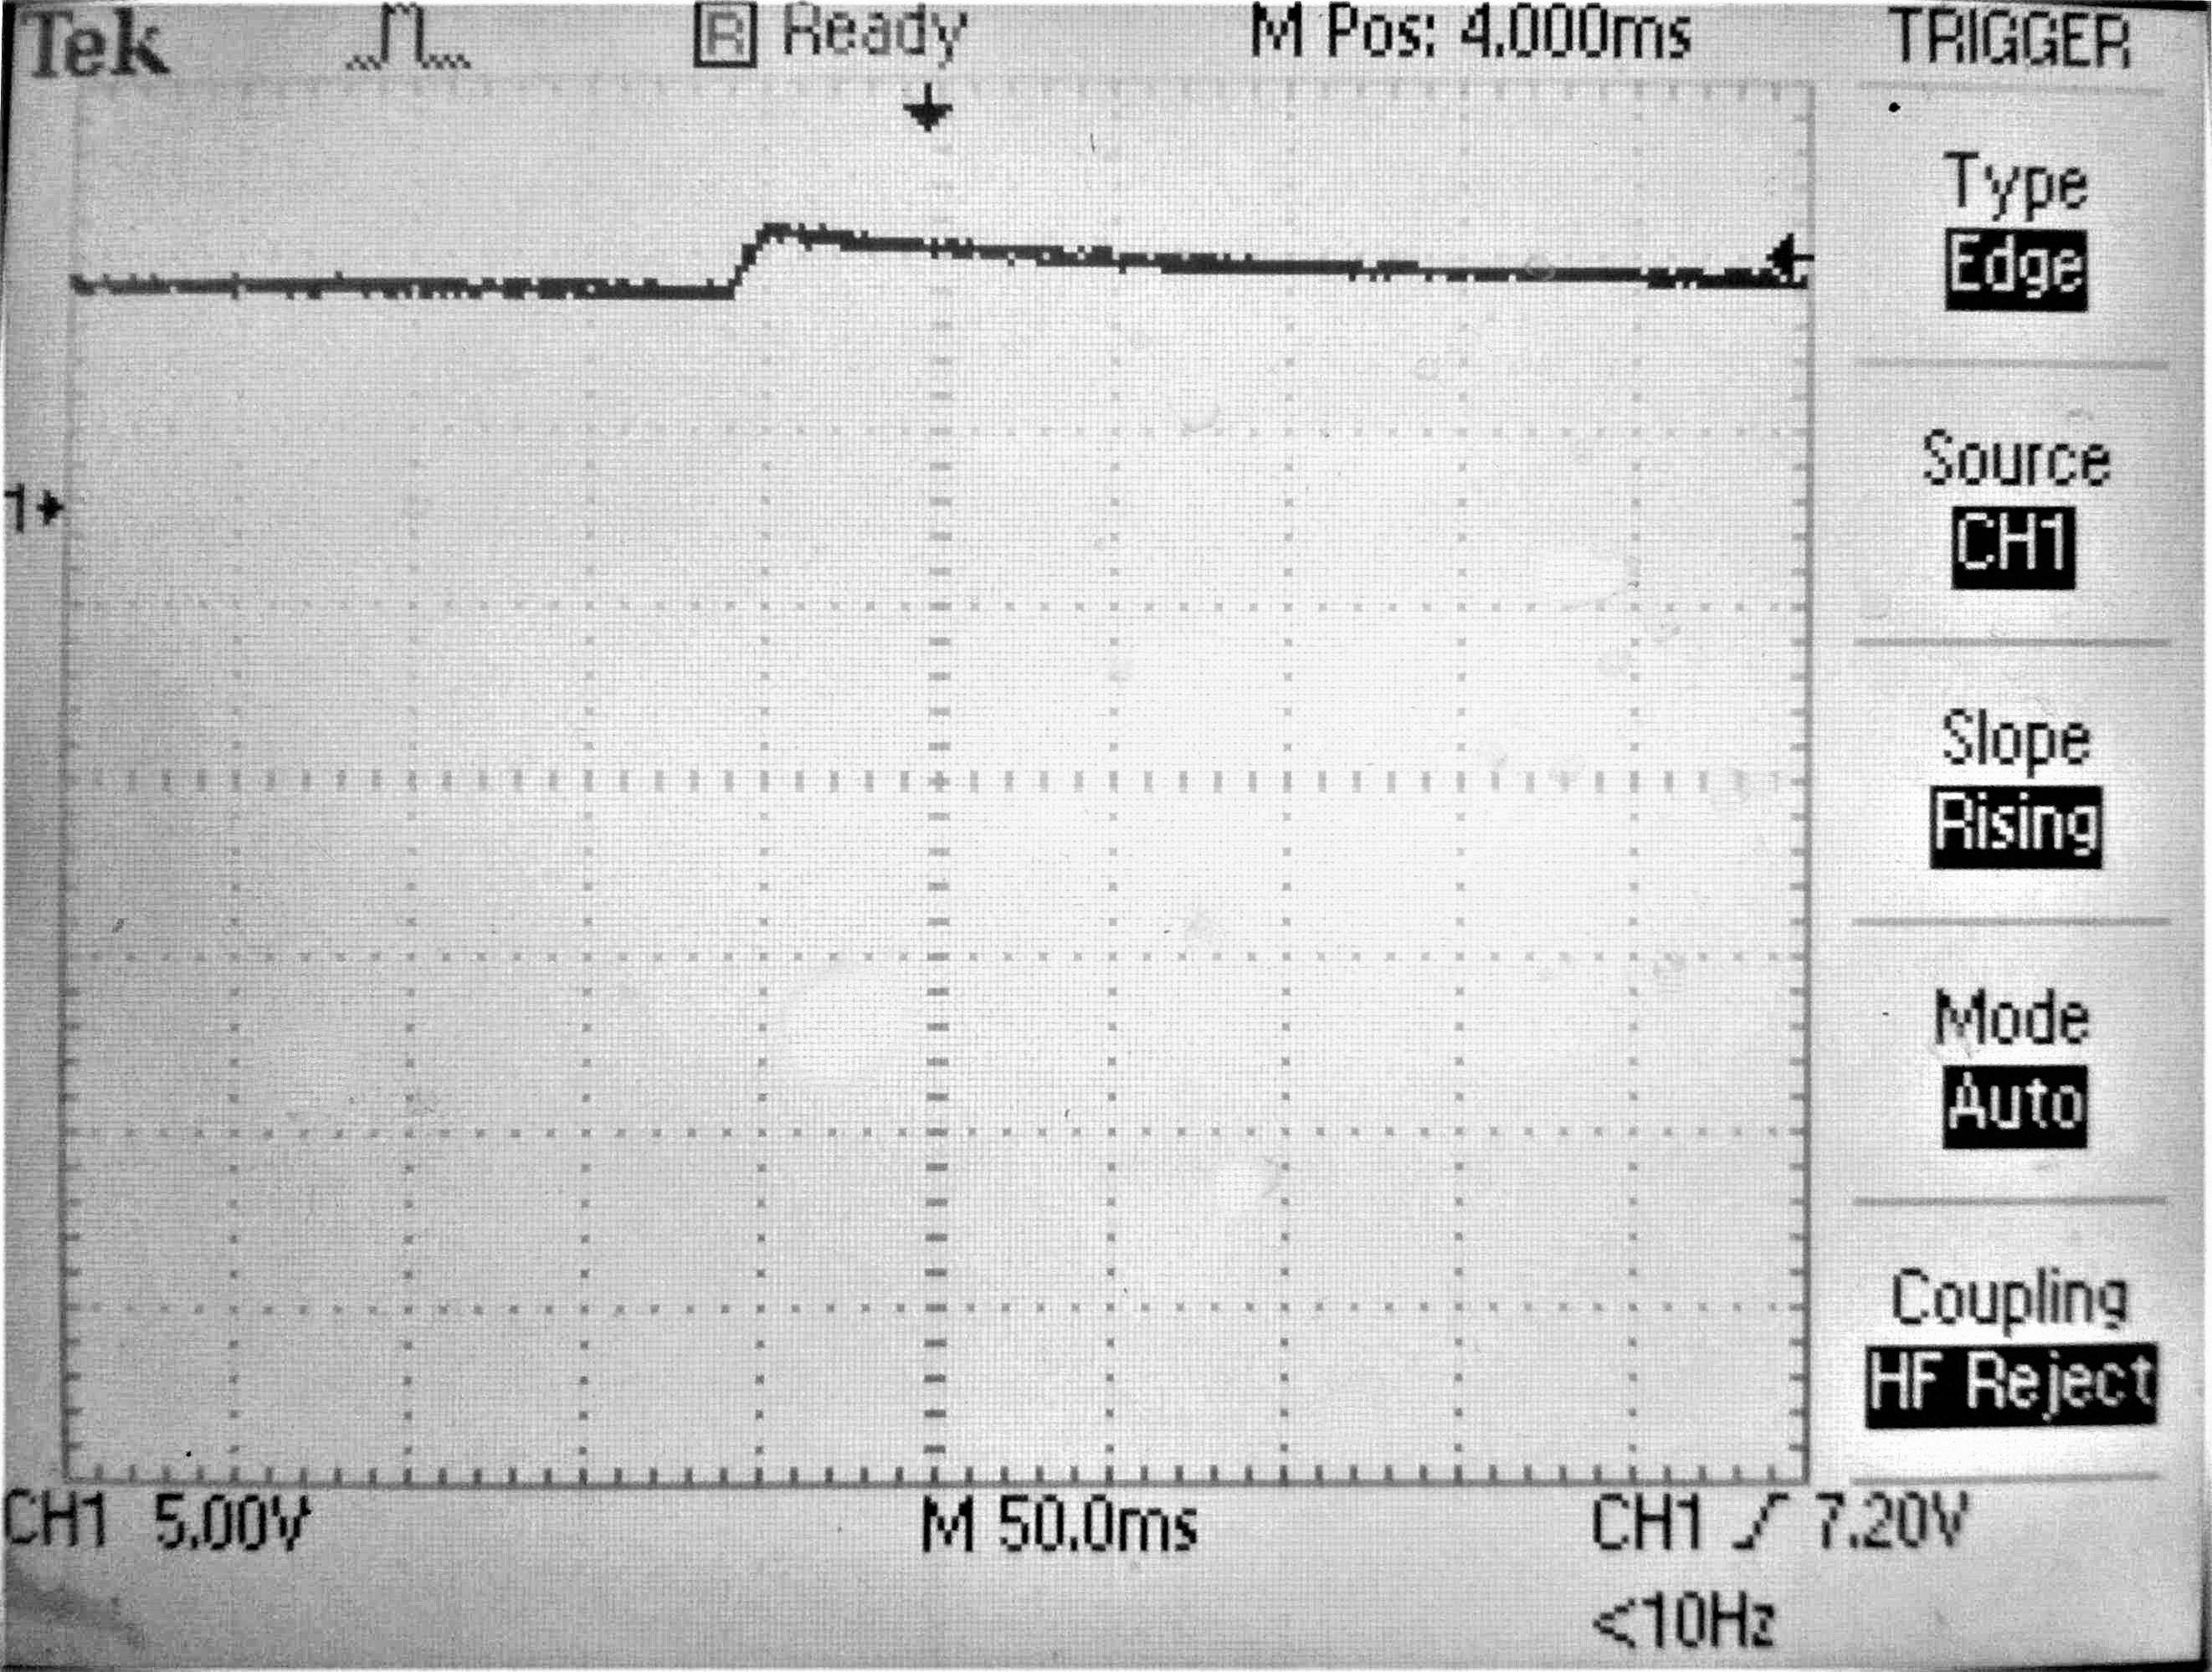
\includegraphics[width=0.39\textwidth]{rys/zasilanieFiltr.jpg}
\end{center}
\end{frame}

\begin{frame}
\frametitle{Elementy indukcyjne w obwodzie}  
\begin{center}
	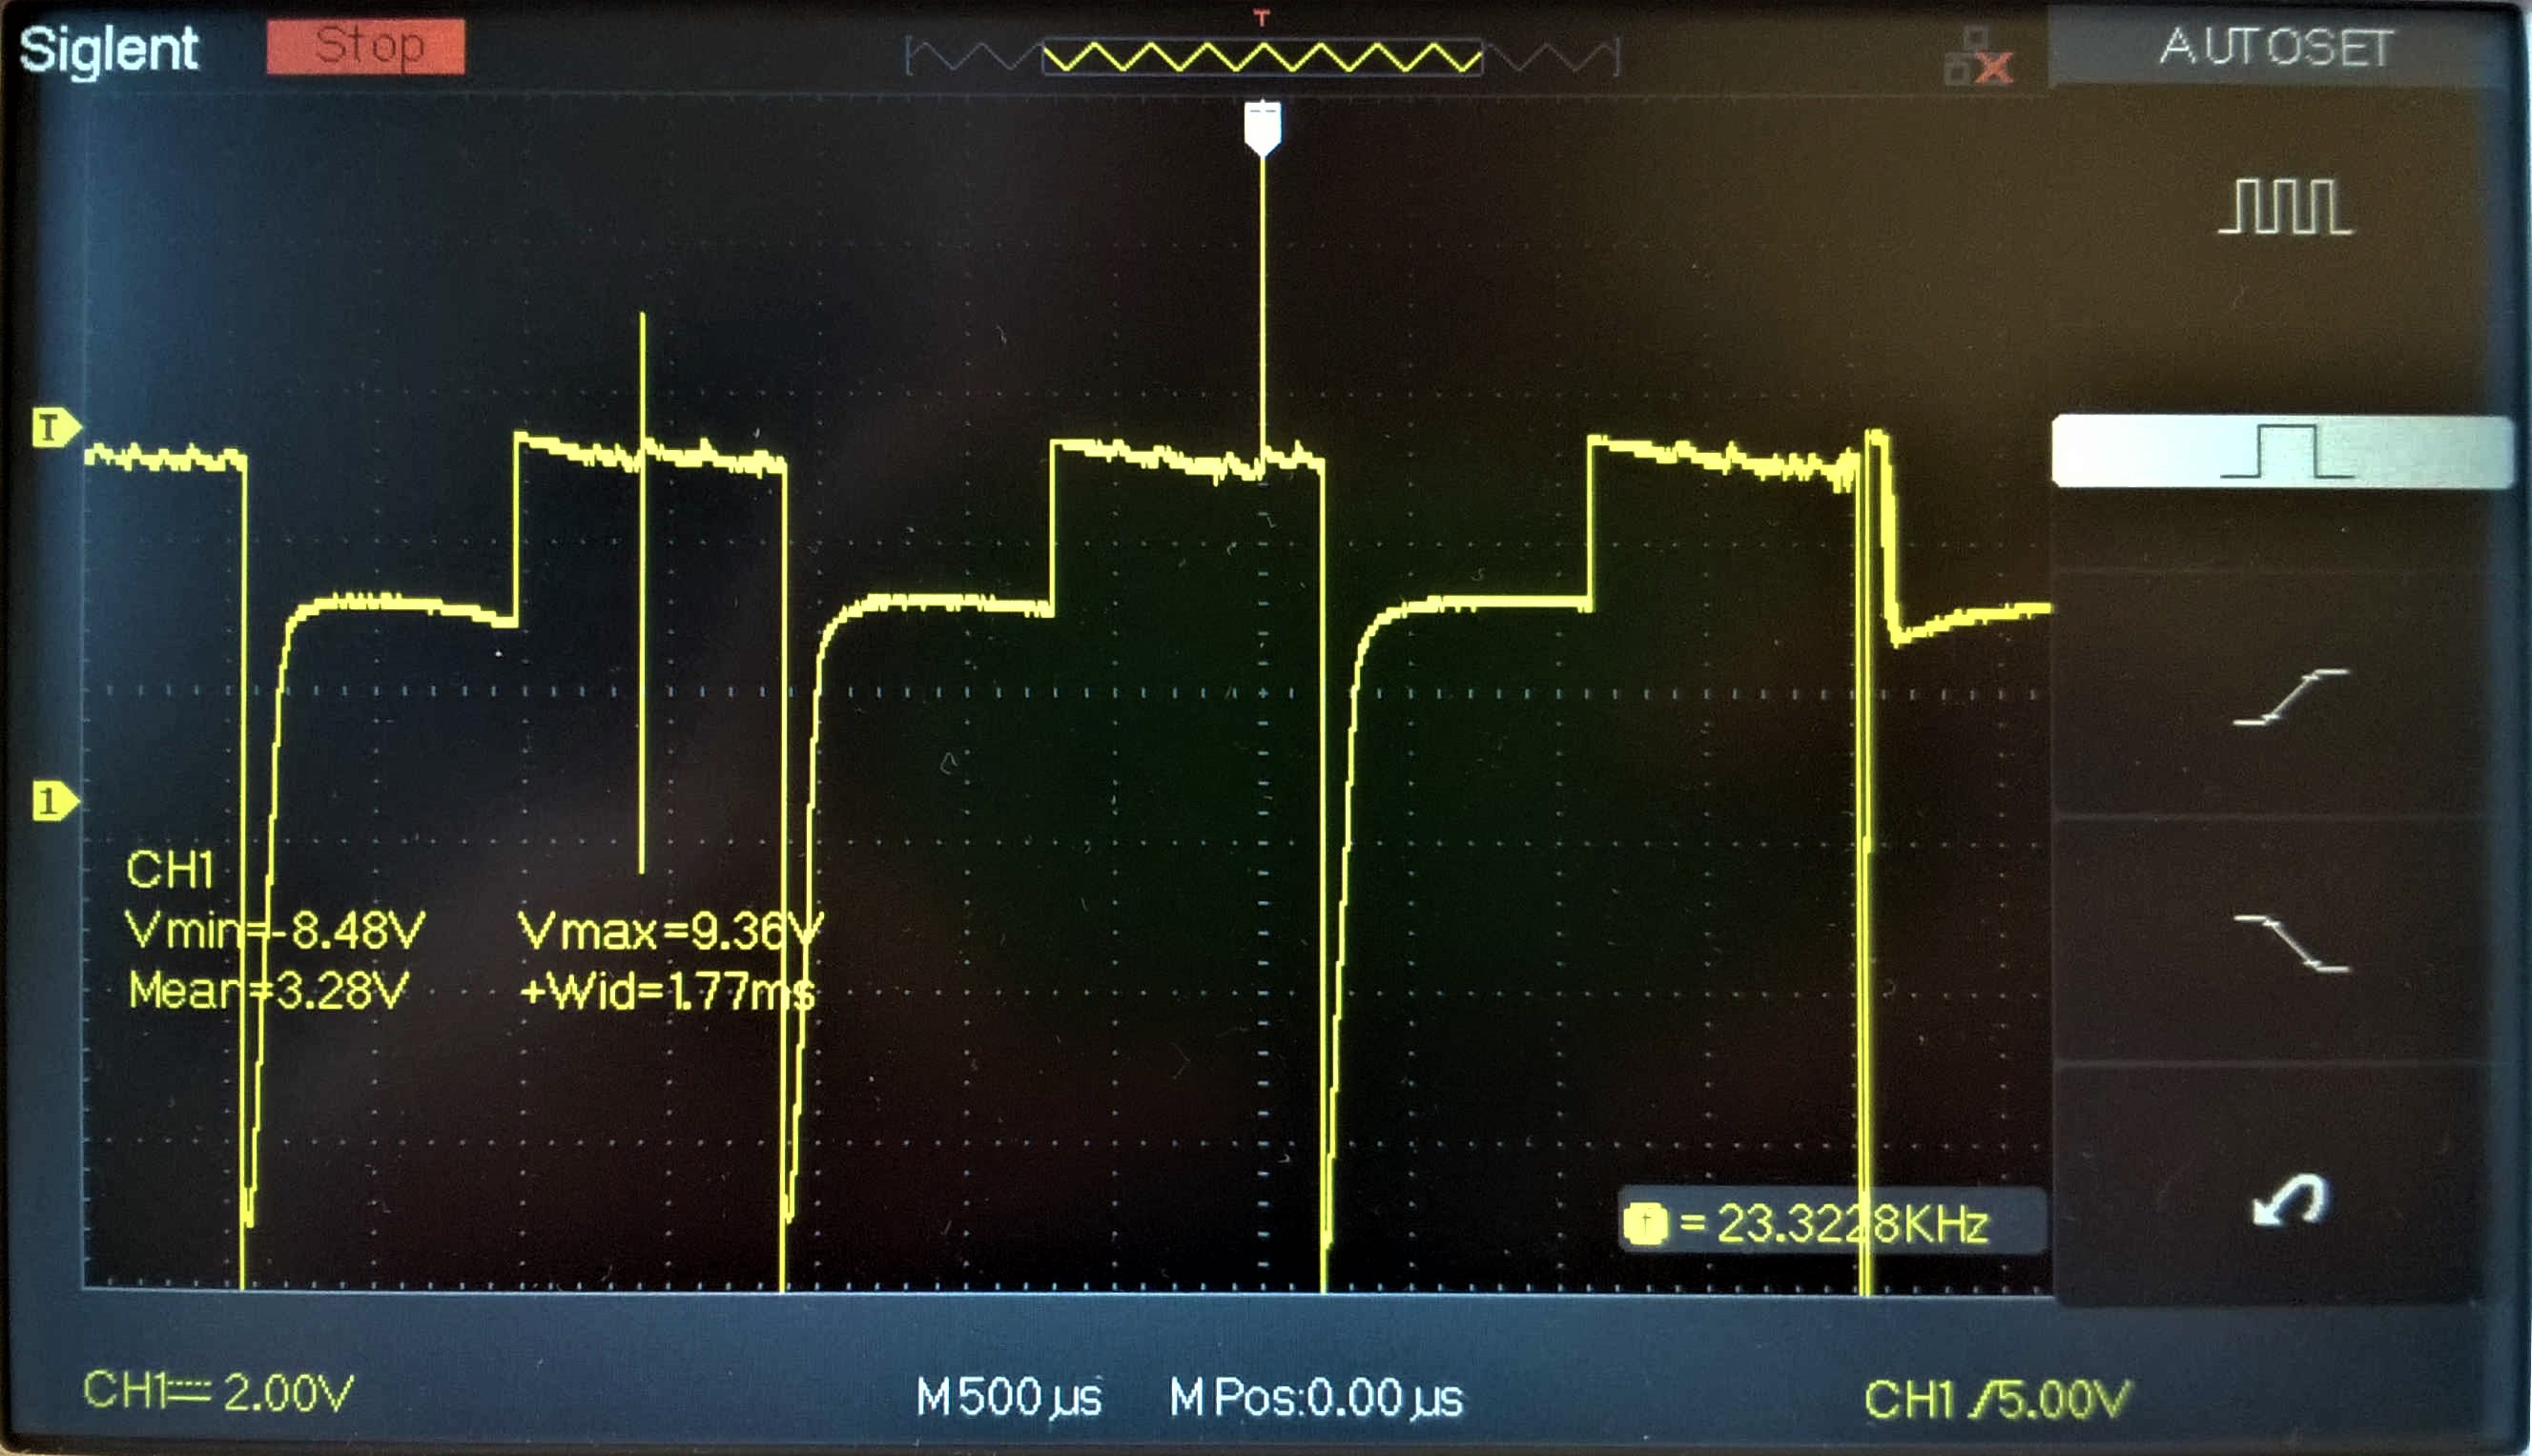
\includegraphics[width=0.5\textwidth]{rys/przedSchottky.jpg}
\end{center}
\begin{center}
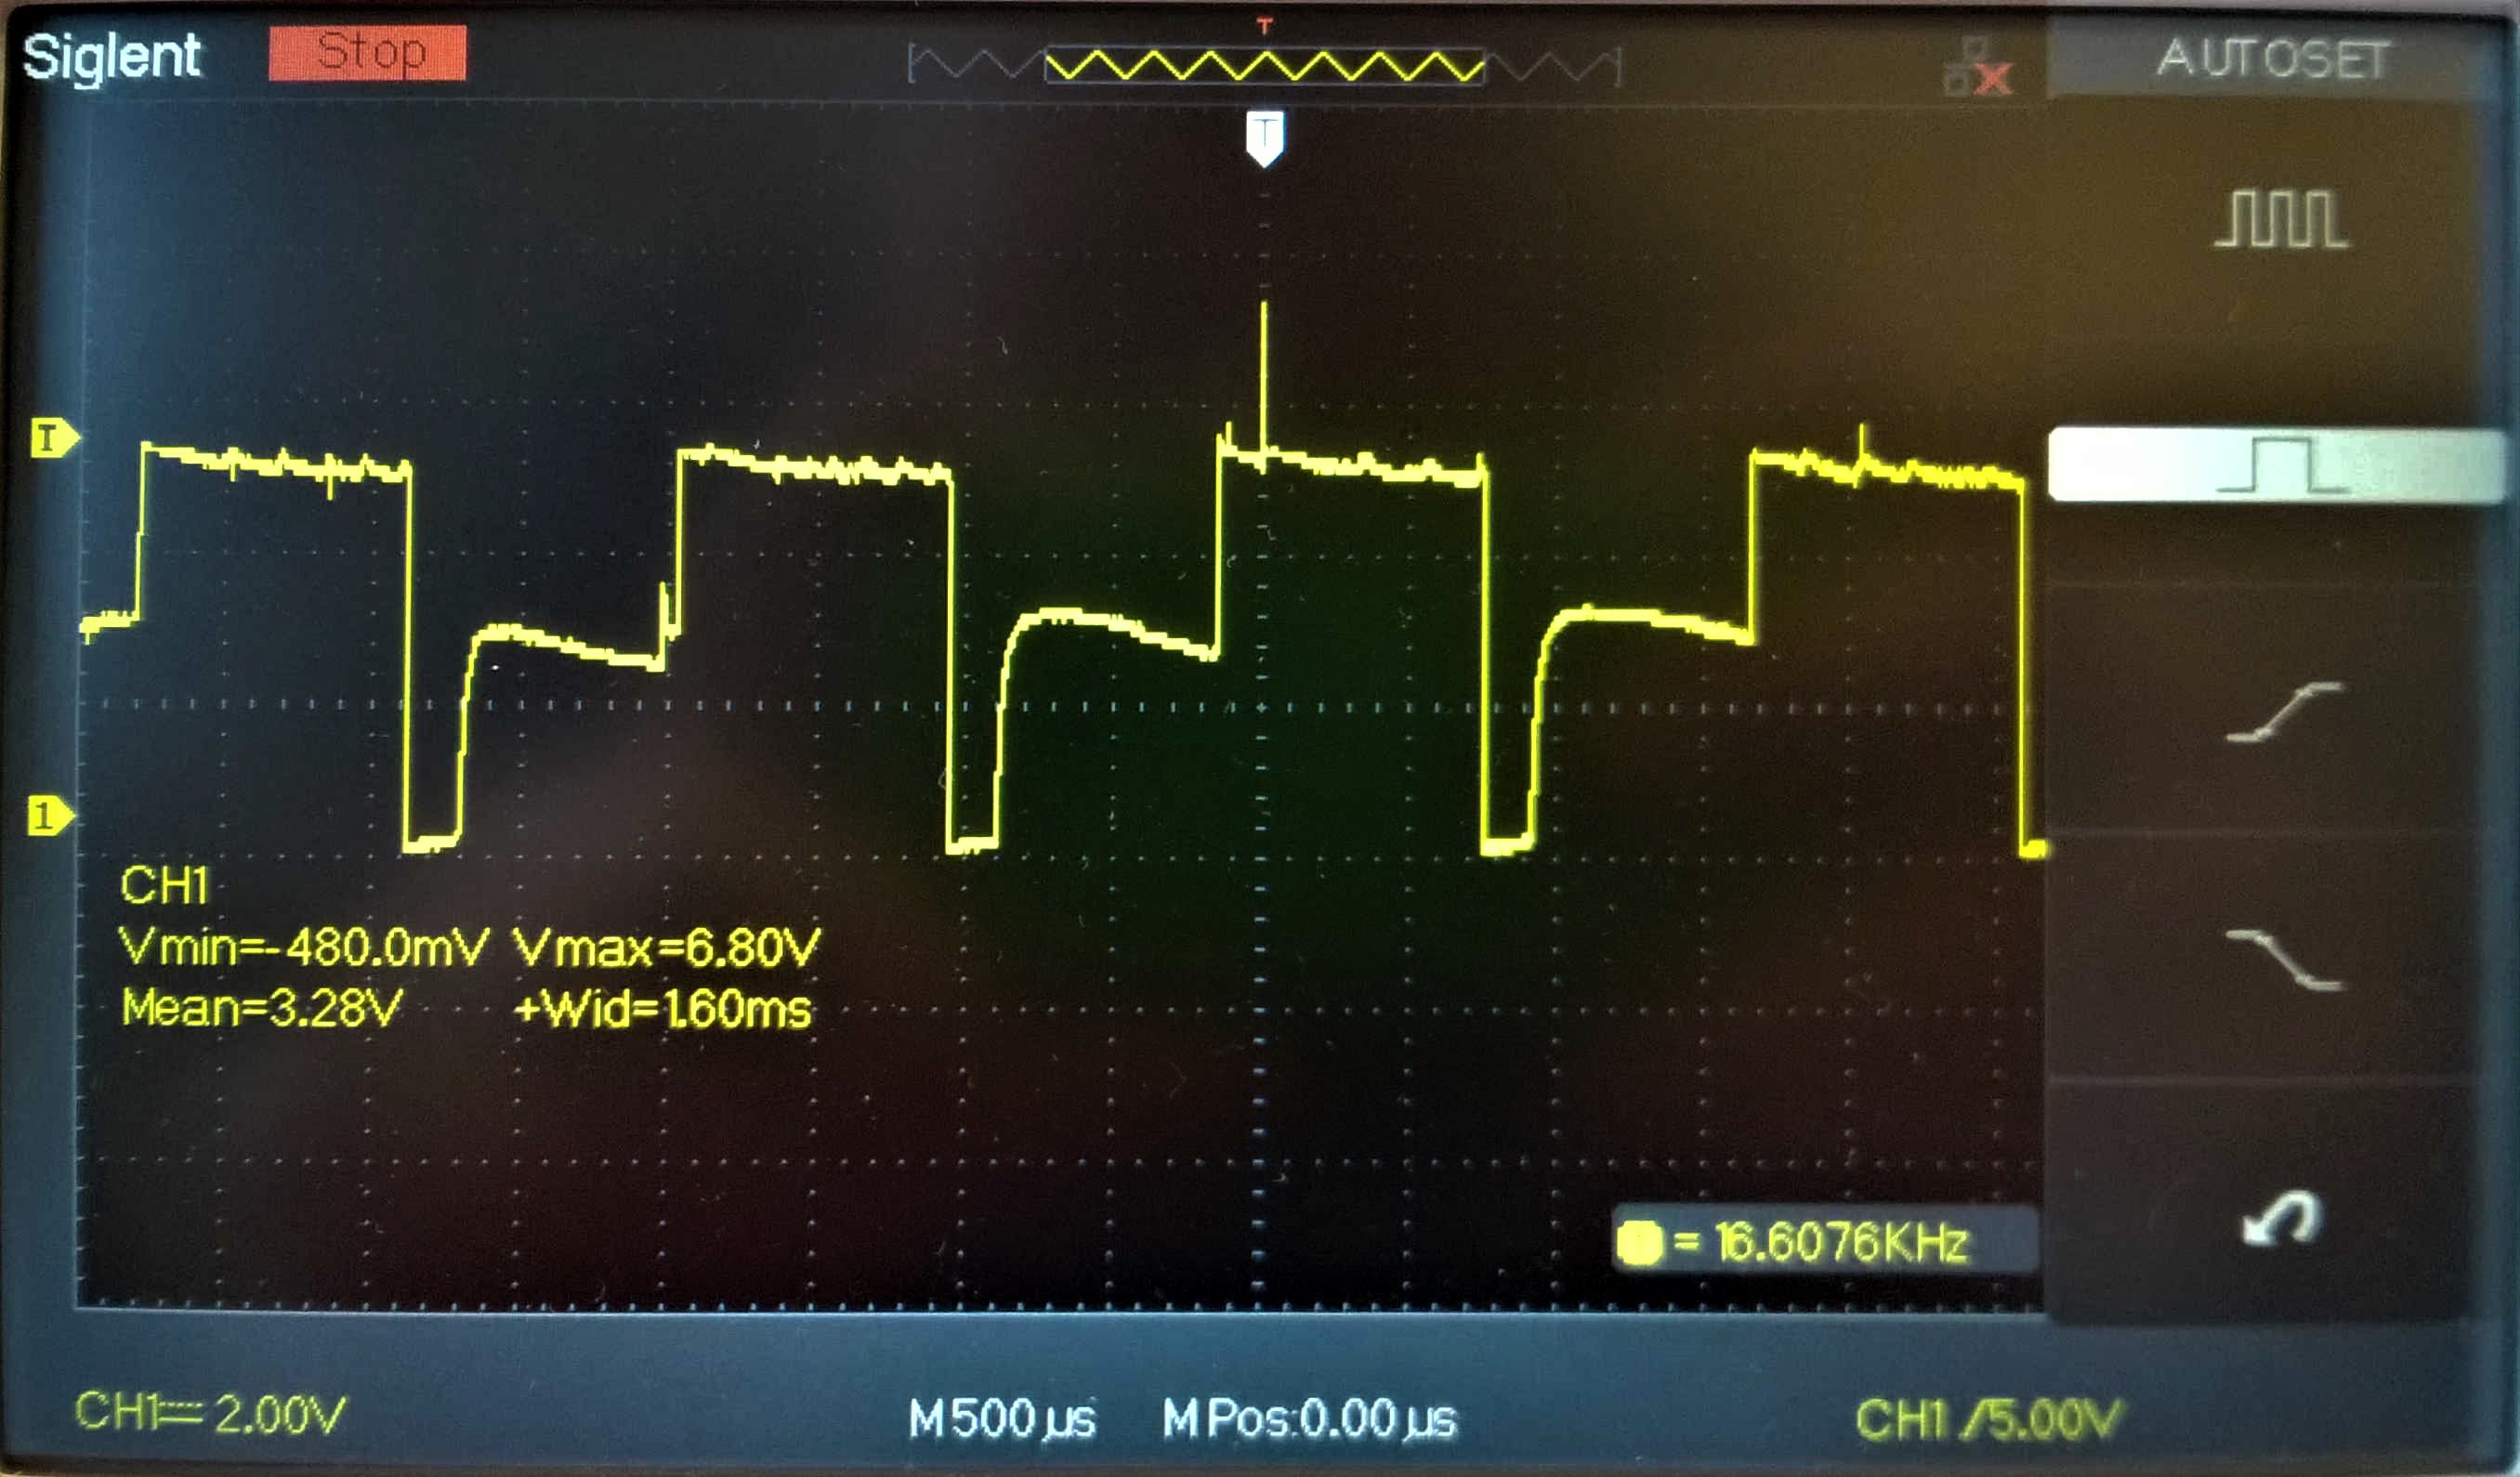
\includegraphics[width=0.49\textwidth]{rys/schottky.jpg}
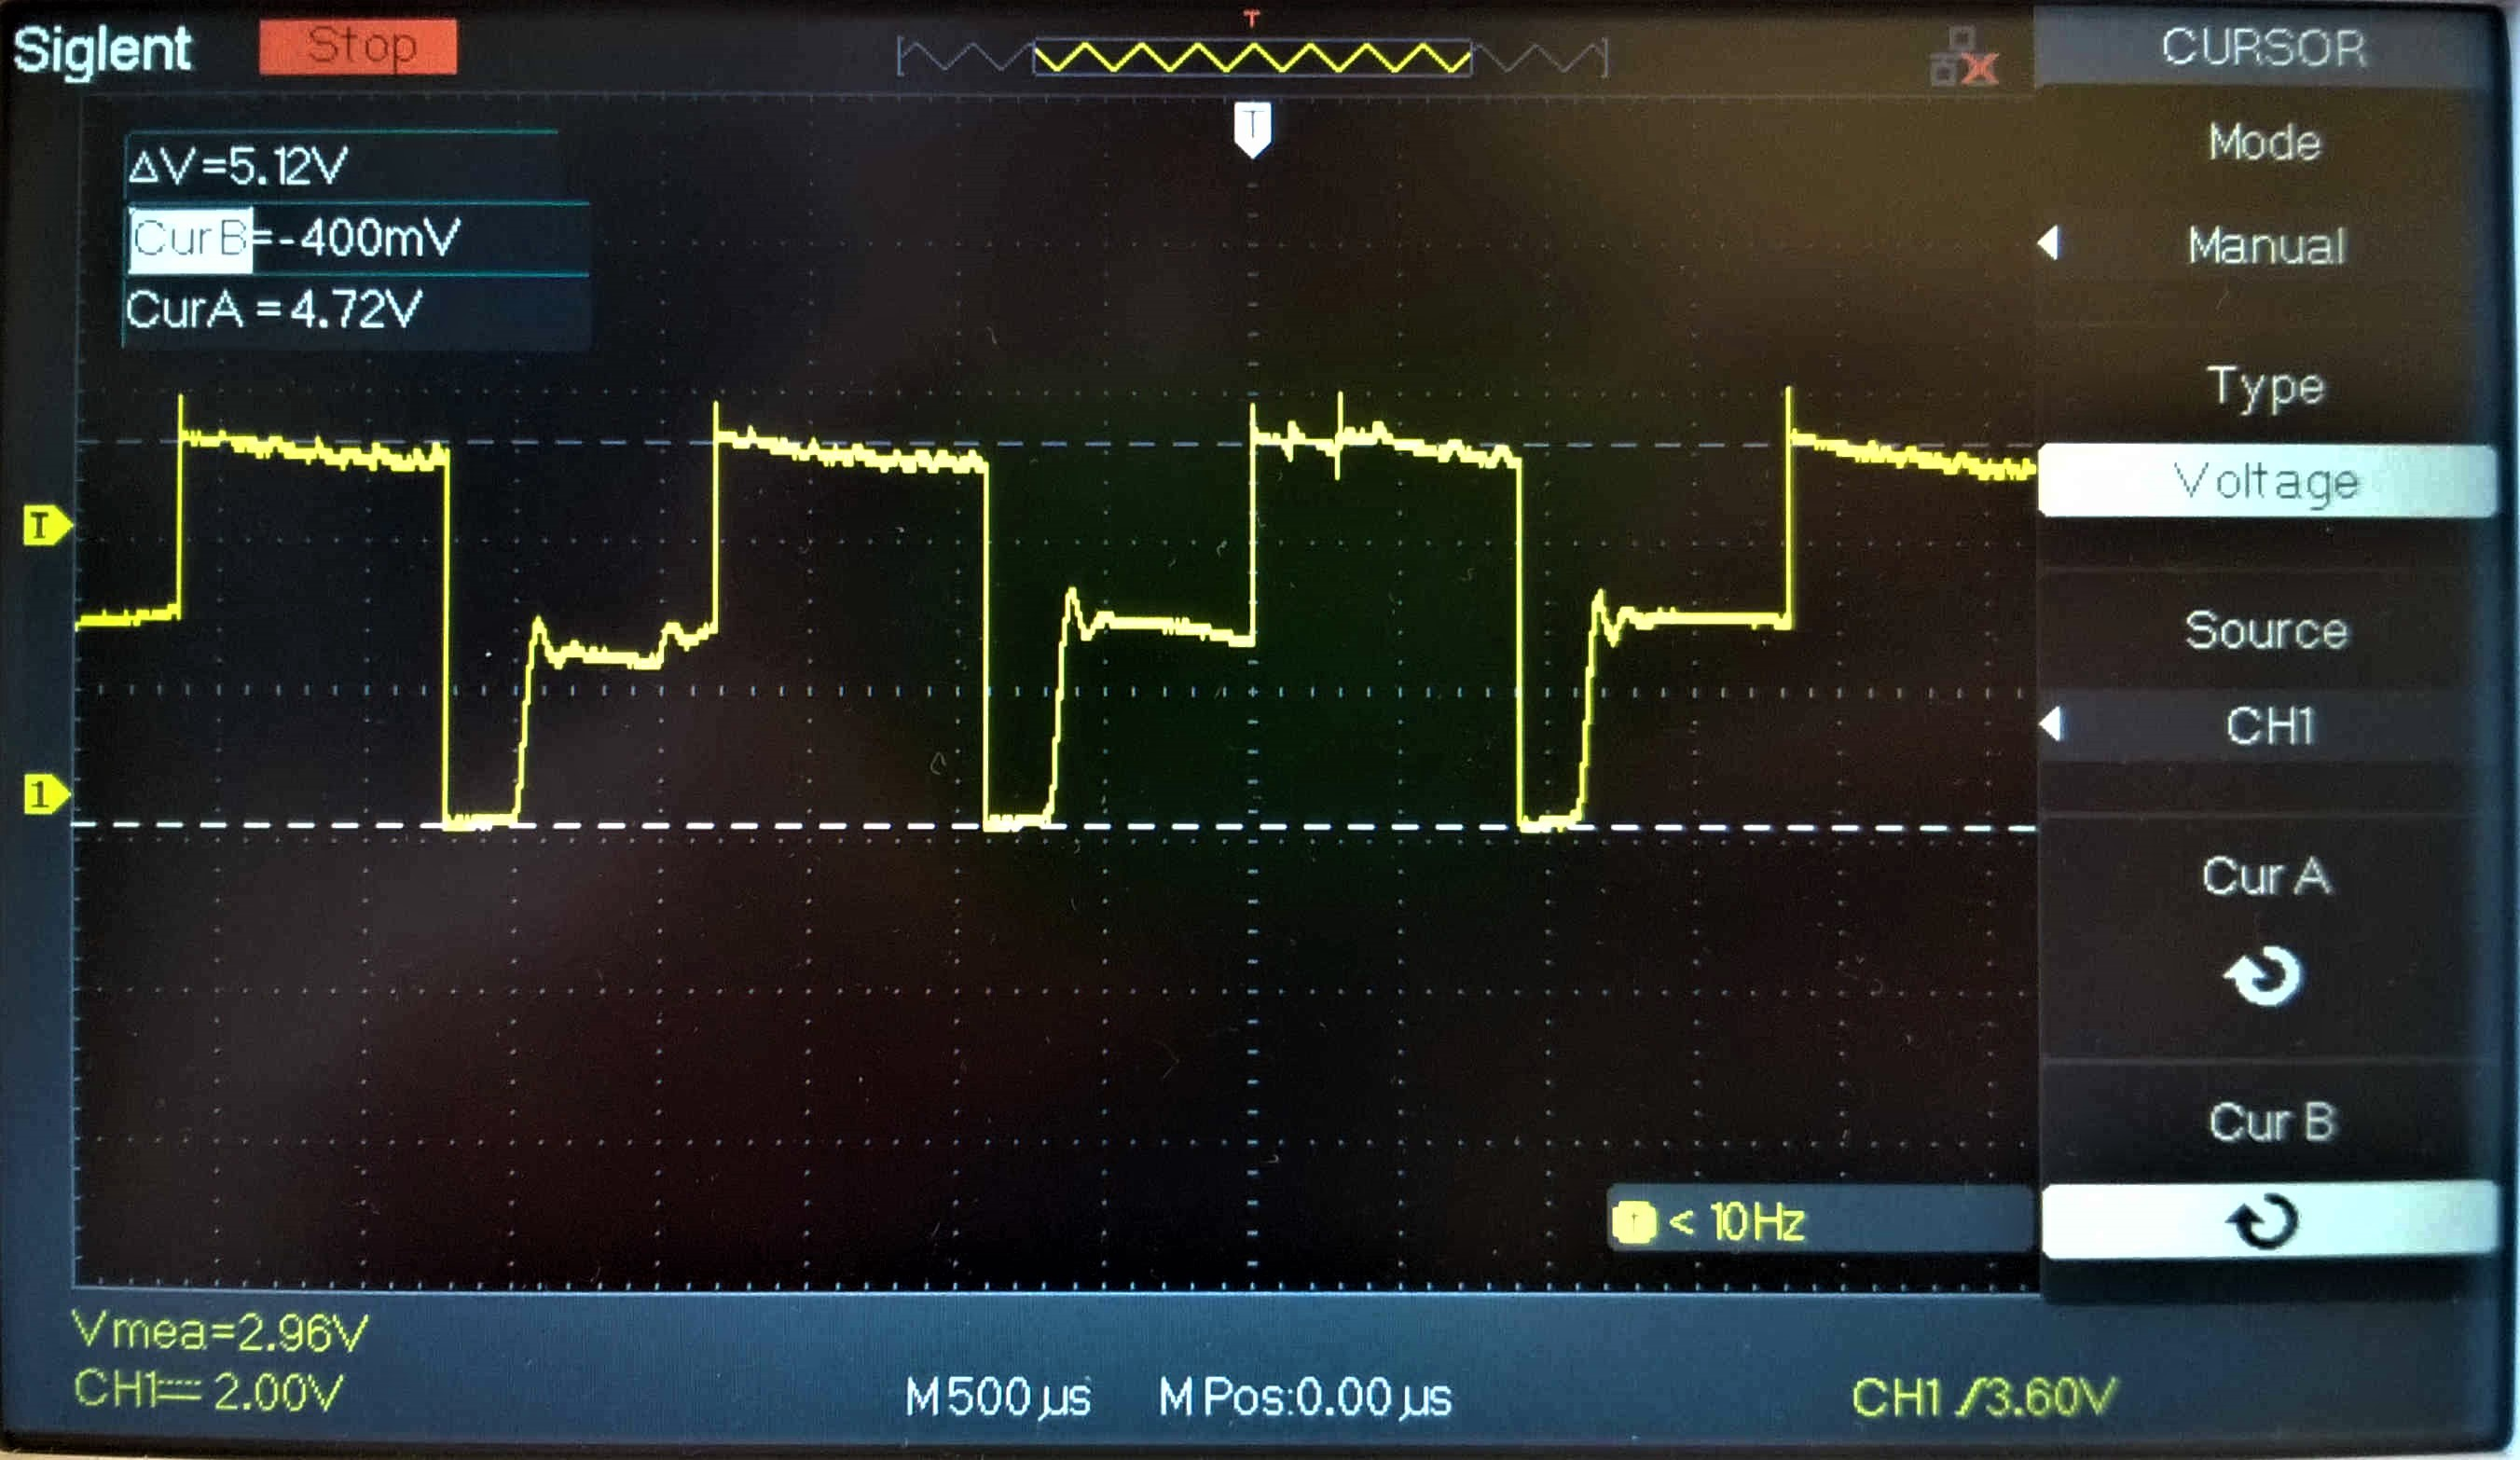
\includegraphics[width=0.49\textwidth]{rys/schottkyZkondem.jpg}
\end{center}
\end{frame}

\section{Program}

		\begin{frame}
		\frametitle{Czas wykonywania obliczeń}
		\tiny
		Porównanie zmiennych dla flagi -O0
		\begin{table}[ht]
			\centering
			\begin{tabular}{|c|c|c|c|}
				\hline
				\multirow{ 2}{*}{\textbf{Numer testu}} & \multicolumn{3}{c|}{\textbf{Czas trwania obliczeń [\si{\milli\second}]}}     \\ \cline{2-4} 
				& \textbf{int} & \textbf{float}   & \textbf{double}      \\ \hline \hline
				1           & 529,446    & 3482,773 & 4332,720     \\ \hline
				2           & 529,470    & 3482,749 & 4332,743     \\ \hline
				3           & 529,467    & 3482,749 & 4332,743     \\ \hline
				4           & 529,469    & 3482,751 & 4332,743     \\ \hline
				5           & 529,467    & 3482,749 & 4332,744     \\ \hline
			\end{tabular}
		\end{table}
			Czas wykonywania pętli. Typ zmiennych -- double. Pętla \SI{100}{razy\per\second} $->$ czas jednej pętli \SI{10}{\milli\second}.
			\begin{table}
			\centering
				\begin{tabular}{|c|c|c|c|}
					\hline
					\multicolumn{4}{|c|}{\textbf{Czas [\si{\micro\second}]}}     \\ \cline{1-4} 
					\textbf{-O0} & \textbf{-Os}   & \textbf{-O3} & \textbf{-Ofast}       \\ \hline \hline
					844    & 452 & 450 & 414     \\ \hline
				\end{tabular}
			\end{table}
			Mimo obiektowego podejścia i "ciężkiego" frameworku wykorzystanie procesora w najgorszym przypadku wynosi od \SI{4.14}{\percent} do \SI{8.44}{\percent}. Czasy pochodzą z zakrętów gdzie jest dużo \texttt{cos} i \texttt{sin}. Można użyć funkcji \texttt{constexpr} i wyliczyć \texttt{Look up table}.
			
			Rozmiar pamięci \texttt{RAM} mikrokontrolera to \SI{20480}{B}, natomiast \texttt{Flash} \SI{65536}{B}.
			\tiny
			\begin{table}
				\centering
				\begin{tabular}{|c|c|c|c|c|}
					\hline
					\multirow{ 2}{*}{\textbf{Pamięć}} & \multicolumn{4}{c|}{\textbf{Wykorzystanie pamięci}}     \\ \cline{2-5} 
					& \textbf{-O0} & \textbf{-Os}   & \textbf{-O3}   & \textbf{-Ofast}     \\ \hline \hline
					\textbf{RAM}         & \SI{22.9}{\percent} (\SI{4696}{B})   & \SI{22.9}{\percent} (\SI{4680}{B}) & \SI{22.9}{\percent} (\SI{4680}{B}) & \SI{22.9}{\percent} (\SI{4680}{B})     \\ \hline
					\textbf{Flash}           & \SI{84.6}{\percent} (\SI{55424}{B})    & \SI{59.0}{\percent} (\SI{38688}{B}) & \SI{62.2}{\percent} (\SI{40736}{B})  & \SI{62.2}{\percent} (\SI{40736}{B})     \\ \hline
				\end{tabular}
			\end{table}
		\end{frame}

	\begin{frame}
	\frametitle{Koniec}
	\centering
	Dziękuję za uwagę
\end{frame}
\end{document}

%%%%%%%%%%%%%%%%%%%%%%%%%%%%%%%%%%%%%%%%%%%%%%%%%%%%%%%%%%%%%%%%%%%%%%%%%%%%% 
% Koniec dokumentu
%%%%%%%%%%%%%%%%%%%%%%%%%%%%%%%%%%%%%%%%%%%%%%%%%%%%%%%%%%%%%%%%%%%%%%%%%%%%% 
